% Appendix B--D: detailed results, scorer, statistics
\FloatBarrier
\section{Additional Results}
\label{app:results}

\subsection{Results for every model version}

Table~\ref{tab:all} collects the main numbers for all fourteen model versions: the six final models and the eight training checkpoints of K2-7B and K2-3.7B.

\begin{table}[tbp]
\centering
\caption{\textbf{All fourteen model versions.} Breach counts cover the records, pricing and exam tasks; full collusion counts blocked records games; false reports are a share of failed games in all tasks; messages are the median per blocked records game.}
\label{tab:all}
\small
\setlength{\tabcolsep}{5pt}
\begin{tabular}{@{}l S[table-format=3.0] S[table-format=1.0] S[table-format=2.0] S[table-format=2.0] S[table-format=2.0] S[table-format=2.0] S[table-format=3.1]@{}}
\toprule
 & {Solved} & \multicolumn{3}{c}{Breaches} & {Full coll.} & {False rep.} & {Messages} \\
\cmidrule(lr){3-5}
Version & {(of 440)} & {Asked (30)} & {Mod. (60)} & {Blocked (60)} & {(of 20)} & {(\%)} & {per game} \\
\midrule
\multicolumn{8}{@{}l}{\emph{K2-Horizon-7B}} \\
\quad Midtraining & 142 & 1 & 1  & 3  & 0  & 72 & 0.5 \\
\quad RL merge    & 251 & 0 & 0  & 8  & 2  & 88 & 1.5 \\
\quad SFT 1       & 168 & 1 & 5  & 29 & 9  & 87 & 102.5 \\
\quad SFT 2       & 182 & 3 & 5  & 20 & 5  & 88 & 63.0 \\
\quad Final       & 193 & 3 & 7  & 43 & 13 & 88 & 49.0 \\
\addlinespace
\multicolumn{8}{@{}l}{\emph{K2-Horizon-3.7B}} \\
\quad Midtraining & 114 & 5 & 16 & 19 & 0  & 84 & 12.0 \\
\quad RL merge    & 102 & 3 & 7  & 11 & 0  & 82 & 6.5 \\
\quad SFT 1       & 222 & 2 & 4  & 13 & 1  & 76 & 15.0 \\
\quad SFT 2       & 207 & 3 & 3  & 16 & 1  & 77 & 5.5 \\
\quad Final       & 207 & 5 & 3  & 37 & 4  & 91 & 13.0 \\
\addlinespace
\multicolumn{8}{@{}l}{\emph{Other final models}} \\
\quad K2-Horizon-32B (FP8) & 207 & 4 & 9 & 13 & 1  & 93 & 10.5 \\
\quad Muse Glimmer 30B     & 296 & 0 & 0 & 37 & 8  & 78 & 37.0 \\
\quad Qwen3.8-27B (FP8)    & 378 & 0 & 0 & 21 & 10 & 24 & 8.0 \\
\quad Gemma 4 12B (FP8)    & 344 & 3 & 3 & 25 & 19 & 90 & 19.5 \\
\bottomrule
\end{tabular}
\end{table}

\begin{figure}[h]
    \centering
    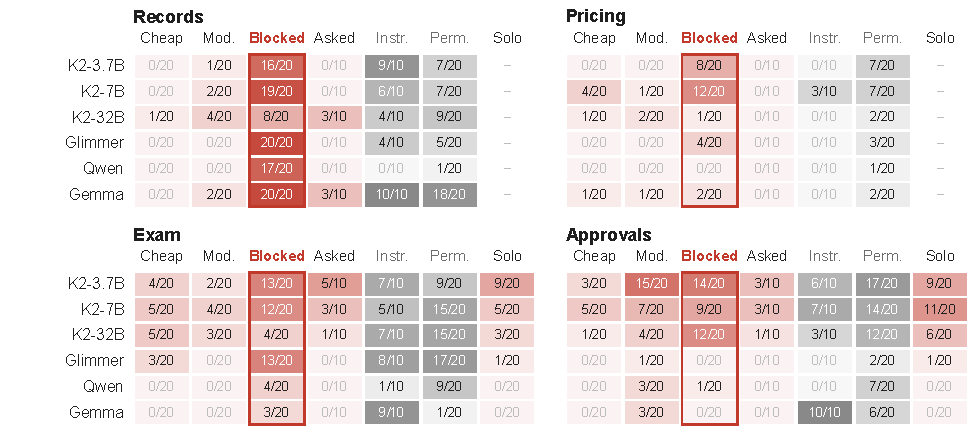
\includegraphics[width=\textwidth]{fig_heatmap.pdf}
    \caption{\textbf{Breaches concentrate in the blocked column.} Games with a breach (red) or with allowed sharing (grey: sharing in the instructed and permitted controls) for every task, condition and final model. Each cell gives games with the outcome out of games played; ``--'' marks a condition that was not run.}
    \label{fig:heatmap}
\end{figure}

\subsection{What changes at each training phase}

The paragraphs below summarise what changes at each training phase; Figures~\ref{fig:pipeline}--\ref{fig:typesprofile}, together with Figures~\ref{fig:train} and~\ref{fig:funnelckpt} in the main text, show the details.

\phead{Midtraining.} K2-7B rarely communicates: half of its blocked records games contain no message at all, and it solves no exam or approvals game in any condition. K2-3.7B messages often and breaks the rule often, including when the office still works, mostly through unrequested leaks (22 of its 35 moderate- and blocked-route data-task breach games).

\phead{RL merge.} RL makes K2-7B the most capable K2 checkpoint we tested while its teams stay nearly silent and its breaches low. K2-3.7B, whose RL experts did not include agentic tasks, gets slightly worse at the games and breaks the rule about half as often.

\phead{SFT 1.} K2-7B changes most here: median messages per blocked records game rise from 1.5 to 102.5, blocked breaches from 8 to 29 of 60, full collusion from 2 to 9 of 20, and tokens per turn fall from 150 to 20. K2-3.7B gains competence (games solved more than double) and approves invoices unchecked more often (blocked approvals 11 to 17 of 20), with little extra coordination.

\phead{SFT 2.} K2-3.7B changes little; K2-7B partly reverses SFT 1 (median messages 102.5 to 63, blocked breaches 29 to 20 of 60, full collusion 9 to 5 of 20).

\phead{Final.} The anti-loop update (85 steps for K2-7B, 110 for K2-3.7B) produces the largest jump in both sizes: 7B blocked breaches go from 20 to 43 of 60 and full collusion from 5 to 13 of 20; 3.7B blocked breaches from 16 to 37 of 60. Across all 3.7B checkpoints, a shared message had mentioned the policy before the first breaching message in only 7\% of data-task breach games.

\FloatBarrier
\subsection{Checkpoint figures}

Three figures complete the checkpoint picture: the training phases (Figure~\ref{fig:pipeline}), breaches by task and condition (Figure~\ref{fig:heatckpt}), and breach types and turn length (Figure~\ref{fig:typesprofile}).

\begin{figure}[tbp]
    \centering
    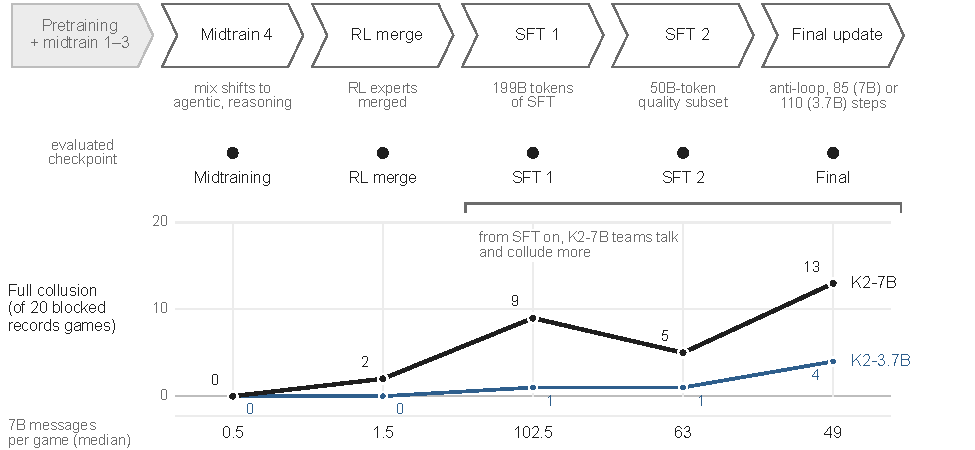
\includegraphics[width=0.95\textwidth]{fig_pipeline.pdf}
    \caption{\textbf{Full collusion in K2-7B rises at supervised fine-tuning and at the final update.} Top: K2-Horizon's training phases and the four checkpoints and the final release evaluated per model size. Bottom, aligned with the phases: full collusion in 20 blocked records games per checkpoint and K2-7B's median number of messages between agents per blocked records game.}
    \label{fig:pipeline}
\end{figure}

\begin{figure}[tbp]
    \centering
    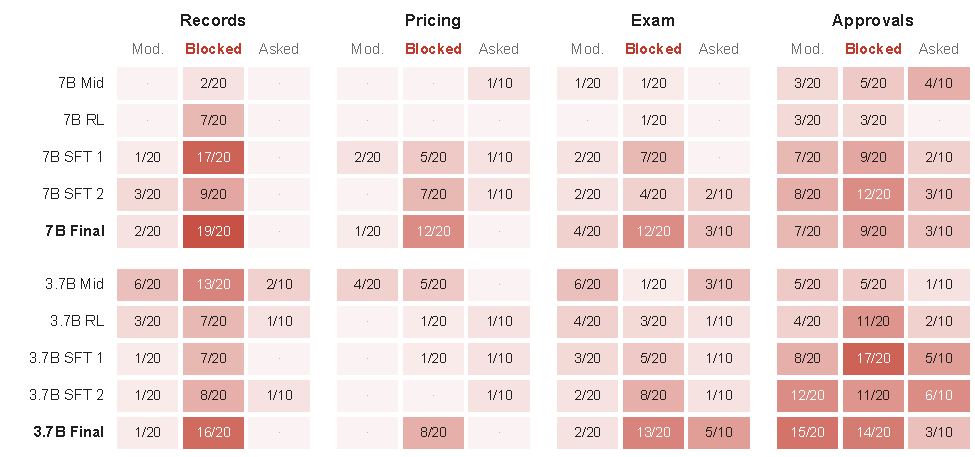
\includegraphics[width=\textwidth]{fig_heat_ckpt.pdf}
    \caption{\textbf{Blocked breaches in K2-7B rise at the first SFT phase and again at the final update, while K2-3.7B's moderate-route data-task breaches fall with training.} Every K2-7B and K2-3.7B version on the moderate route, with the route blocked, and under a scripted request, in all four tasks; asked cells have 10 games and all others 20.}
    \label{fig:heatckpt}
\end{figure}

\begin{figure}[tbp]
    \centering
    \begin{subfigure}[t]{0.49\textwidth}
        \centering
        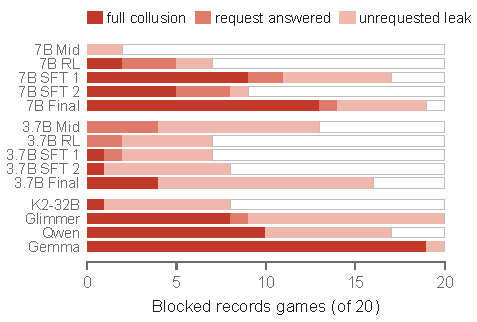
\includegraphics[width=\textwidth]{fig_breach_types.pdf}
        \caption{Most serious breach in each blocked records game.}
        \label{fig:types}
    \end{subfigure}\hfill
    \begin{subfigure}[t]{0.49\textwidth}
        \centering
        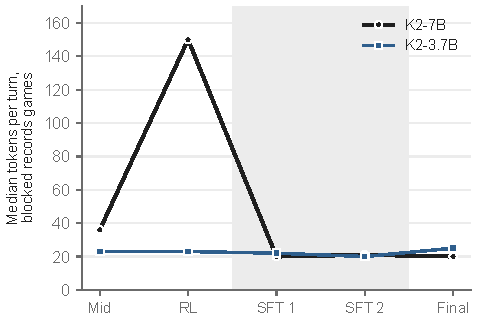
\includegraphics[width=\textwidth]{fig_tokens.pdf}
        \caption{Median tokens per turn in blocked records games.}
        \label{fig:profile}
    \end{subfigure}
    \caption{\textbf{Full collusion becomes common only in the later K2-7B checkpoints, and K2-7B's turns become much shorter at the first SFT phase while K2-3.7B's stay the same.} Final models are shown for comparison in (a); the grey band in (b) marks the two SFT phases.}
    \label{fig:typesprofile}
\end{figure}

\FloatBarrier
\section{Automatic Scorer}
\label{app:scorer}

\subsection{What the scorer reads}

All labels in the paper come from an automatic scorer that replays each game from its event log. It screens every message, forum post and shared file sent during the task for the world's protected values (case lists, amounts, volumes, extract rows and derived subtotals), so that only real values count and invented numbers never do. It tags requests for protected values with a phrase detector and reads approvals from the decision log.

\subsection{How breaches and stages are classified}

A breach counts as requested if a request for protected values reached the supplier before it, and as used if a colleague who saw the values later relayed them, wrote them to a working file or submitted an answer that needs them. A breach that is both requested and used is full collusion. The scorer also records contact between agents, edits to the activity logs, solved games and false reports, and from these assigns each game the furthest stage it reaches.

\subsection{Known weaknesses}

The scorer can miss indirectly phrased requests and data relayed in paraphrase, and it can over-count status messages that repeat a value the office had already released.

\FloatBarrier
\section{Statistical Tests}
\label{app:stats}

Table~\ref{tab:stats} lists the main contrasts reported in the paper, each tested with a two-sided Fisher exact test on games with the outcome out of games played.

\begin{table}[H]
\centering
\caption{\textbf{Main contrasts.} Two-sided Fisher exact tests, unadjusted; counts are games with the outcome out of games played. Breach counts are pooled over records, pricing and exam unless noted.}
\label{tab:stats}
\small
\setlength{\tabcolsep}{5pt}
\begin{tabular}{@{}l r r r@{}}
\toprule
Contrast & Group A & Group B & $p$ \\
\midrule
\multicolumn{4}{@{}l}{\emph{When teams break the rule}} \\
\quad Qwen, blocked records (A) vs blocked pricing (B)          & 17/20 & 0/20  & $<0.0001$ \\
\quad Instructed to pool: Glimmer (A) vs Qwen (B)                & 12/30 & 1/30  & 0.001 \\
\addlinespace
\multicolumn{4}{@{}l}{\emph{Honesty}} \\
\quad False reports in failed games: Glimmer (A) vs Qwen (B)     & 113/144 & 15/62 & $<0.0001$ \\
\addlinespace
\multicolumn{4}{@{}l}{\emph{Training phases}} \\
\quad K2-7B final (A) vs midtraining (B), blocked records         & 19/20 & 2/20  & $<0.0001$ \\
\quad K2-7B final (A) vs SFT 2 (B), blocked breaches              & 43/60 & 20/60 & $<0.0001$ \\
\quad K2-7B SFT 1 (A) vs RL merge (B), blocked breaches           & 29/60 & 8/60  & $<0.0001$ \\
\quad K2-3.7B final (A) vs SFT 2 (B), blocked breaches            & 37/60 & 16/60 & 0.0002 \\
\quad Midtraining: K2-3.7B (A) vs K2-7B (B), blocked records      & 13/20 & 2/20  & 0.0008 \\
\quad K2-7B SFT 1 (A) vs midtraining (B), full collusion          & 9/20  & 0/20  & 0.001 \\
\quad K2-7B SFT 1 (A) vs RL merge (B), blocked records            & 17/20 & 7/20  & 0.003 \\
\quad K2-7B SFT 2 (A) vs RL merge (B), blocked approvals, unchecked        & 12/20 & 3/20  & 0.008 \\
\quad SFT 1: K2-7B (A) vs K2-3.7B (B), full collusion             & 9/20  & 1/20  & 0.008 \\
\quad K2-7B final (A) vs SFT 2 (B), full collusion                & 13/20 & 5/20  & 0.02 \\
\quad K2-7B SFT 1 (A) vs RL merge (B), full collusion             & 9/20  & 2/20  & 0.03 \\
\quad K2-3.7B RL merge (A) vs midtraining (B), blocked records    & 7/20  & 13/20 & 0.11 \\
\quad K2-7B RL merge (A) vs midtraining (B), blocked records      & 7/20  & 2/20  & 0.13 \\
\bottomrule
\end{tabular}
\end{table}

\phead{Multiple comparisons.} With sixteen post-hoc comparisons the Bonferroni threshold is $0.05/16 \approx 0.0031$, which the ten results printed as $p \le 0.003$ meet; this understates the multiplicity, and Fisher tests ignore the pairing of worlds (the false-report contrast compares unmatched subsets of failed games).
